\chapter{Application}
\label{chap:molecules}
\section{Introduction}

With the new suite of tools implemented in \texttt{fromage}, we now focus on applying them to increasingly diverse systems, in the hope to glean some chemical insight. The objective is both to provide robustness to the program, whilst studying the properties of emissive organic molecular crystals .

To fully control the luminescent behaviour of these materials, the excited state radiative and non-radiative decay channels of the molecule need to be understood within a particular condensed phase environment. Despite the abundance in experimental and theoretical investigations of the excited states of molecular crystals, understanding these decay channels is still extremely challenging, and is done on a case-by-case basis for newly discovered compounds. The main obstacle to generalising design rules for these materials is the interconnectedness of their defining properties at the molecular and intermolecular levels.

In this chapter, we analyse the role of different factors affecting the emissive response of thirteen luminescent molecular crystals, which have previously been characterised experimentally (Figure \ref{fig:molecules_app}). We aim to consider a large enough variety of systems that comparisons can be drawn between crystals with different degrees of packing and chemical similarity. \miguel{Our main focus is to rationalise the Quantum Efficiency of Fluorescence (QEF) of these materials as a competition between radiative and nonradiative decay channels, arising from different inter- and intramolecular factors. We consider a diverse enough range of materials to highlight how differently behaving solute molecules can arrive at the same desirable emissive property in the crystal phase.}

\begin{figure}
\centering
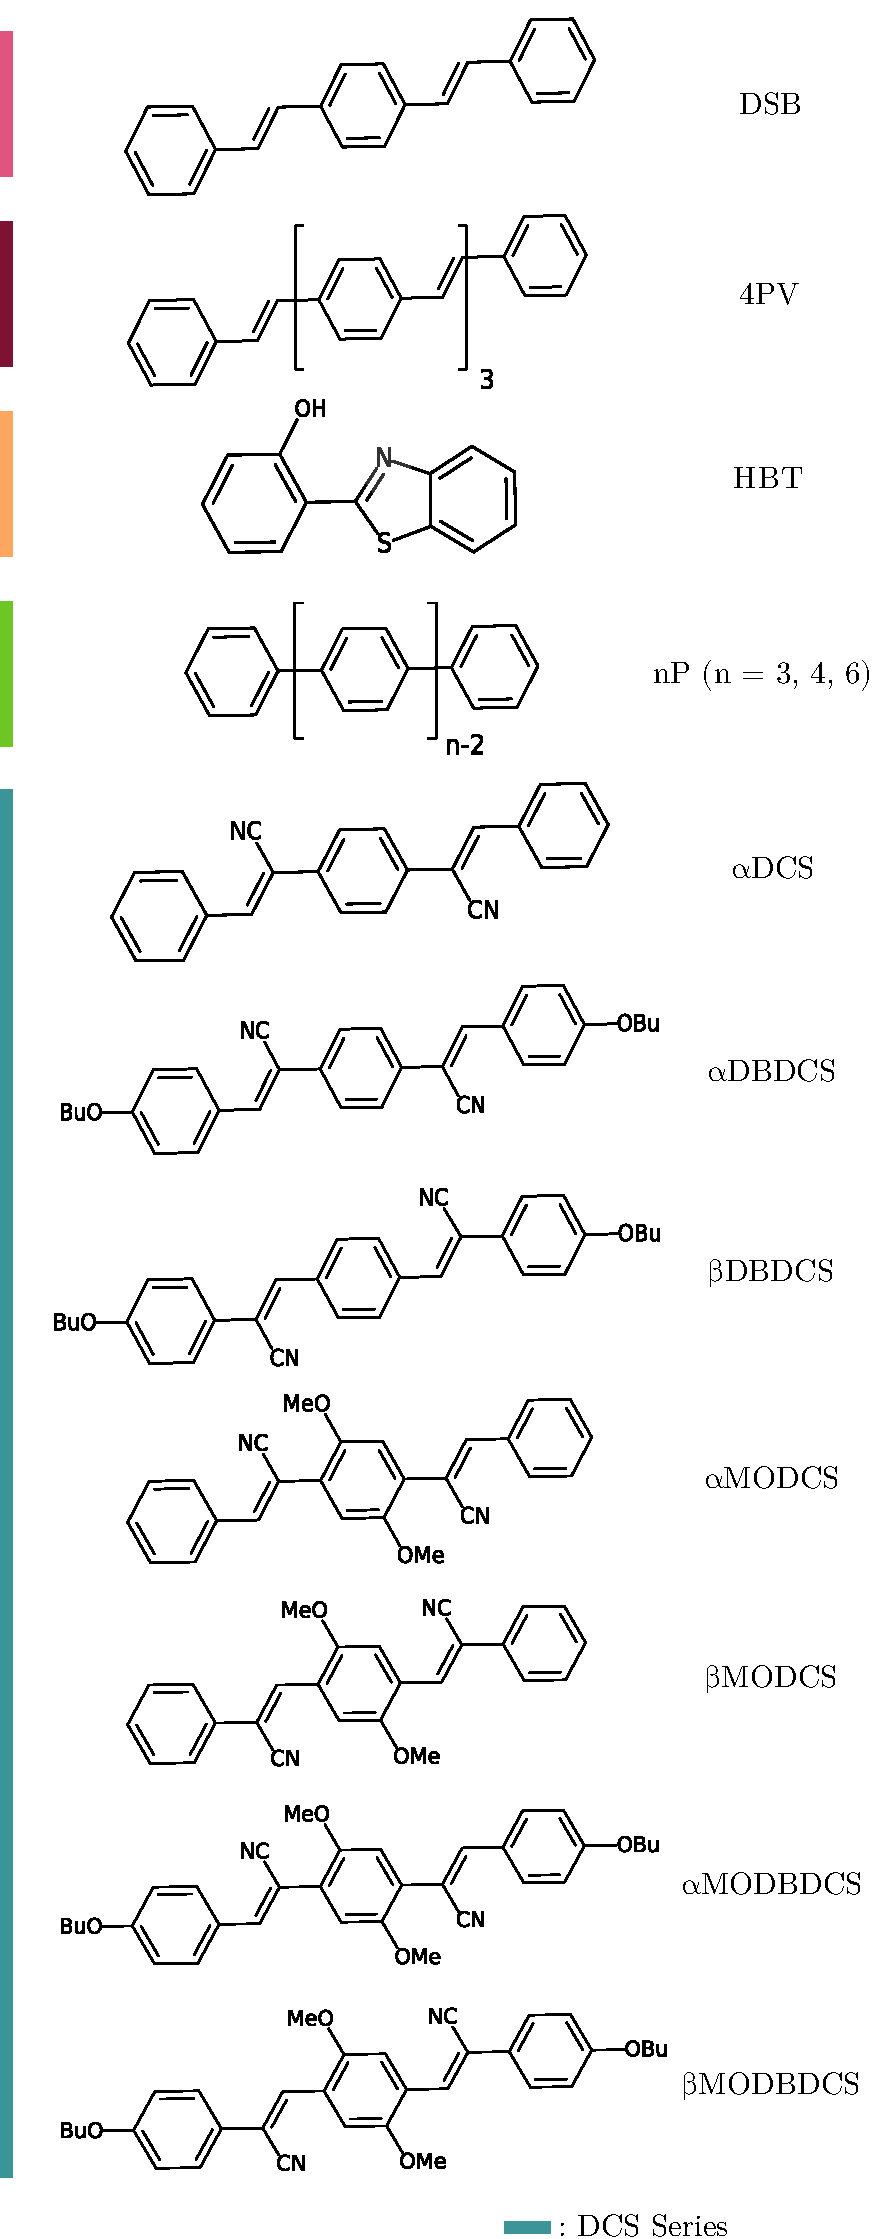
\includegraphics[width=9cm]{Chapters/7Applications/molecules.pdf}
\caption{Molecular structures of the studied systems.}
\label{fig:molecules_app}
\end{figure}
%%%

The crystals were gathered into series based on their backbone structures and substituents. p-oligophenylenes ($n$P, $n$=3, 4, and 6) are a family of organic $\pi-$conjugated molecules composed of phenyl-rings attached to each other via single bonds in para-positions. The DCS series where three phenylene units are connected by vinylene bridges with cyano-group substituents, and additional buthoxy and methoxy groups are added to the backbone. We also consider the DSB molecule, which shares the same backbone but has no substituents and 4PV which further extends the phenylene chain by two phenylene units. Additionally, we consider 2-(2'-hydroxyphenyl)benzothiazole (HBT), a molecule exhibiting excited state proton transfer in the solid state. All molecules are represented on Figure \ref{fig:molecules}.

% Bogatko2016 says that the absorption of acenes goes down with length

Barring certain substitutions of the DCS family and HBT, all systems display amplified spontaneous emission (ASE) in crystal, making them candidates for use as organic single crystal lasers, as detailed in Reference \citenum{Gierschner2016}. All molecules undergo Solid State Luminescence (SSL),\cite{Shi2017} some of it induced by crystallisation\textemdash{}Solid State Luminescence Enhancement (SLE).


%%%

%%Throwing some ideas around
We first present the computational details of our findings. Then, in order to understand the emissive behaviour of the crystals, we analyse  the geometric features of the crystal packing, the excitonic coupling between constituent dimers, and the energetics of the excited states along critical points of their potential energy surfaces. We conclude by comparing the findings between series and assessing the efficacy of our available analysis methods in \miguel{elucidating competing radiative and nonradiative mechanisms}.


\section{Computational Details}
The crystal structure geometries were optimised using PBE-D2 as implemented in \texttt{Quantum Espresso}\cite{Giannozzi2009}, with a basis set cut-off of 50 Ry and various Monkhorst-Pack Grids chosen in accordance with the unit cell shapes.

The investigation of the multiple molecules was facilitated by the recent development of \texttt{fromage}, a Python library dedicated to studying excited state molecular aggregates and crystals. This work showcases the robustness of its features by applying geometry analysis tools, excitonic coupling evaluation, and ONIOM methods to the crystals.

In order to isolate dimers from the lattice, a spherical molecular cluster was extracted from the crystal, and its pairs of molecules with with intermolecular contacts smaller than 4 \AA{} were selected. Then, the intermolecular atomic distances of each dimer were evaluated and sorted so as to provide a fingerprint for the dimer configuration. These distances were finally compared between dimers and if their RMSD fell below $10^{-4}$ \AA, the dimers were considered identical and only one was preserved.

To characterise the configurations of the unique dimers, an orthonormal pair of principal and secondary axes was calculated for each constituent fragment, and the angles between same axes of two molecules was evaluated. To obtain the vectors, first, all atoms of the molecule were projected onto an averaged plane via singular value decomposition. The principal axis was defined as the vector tracing the longest interatomic distance and the secondary axis its perpendicular vector on the averaged plane.\cite{Rivera2020} This process is represented for a dimer of the 3P crystal in Figure \ref{fig:axes}.

\begin{figure}
\centering
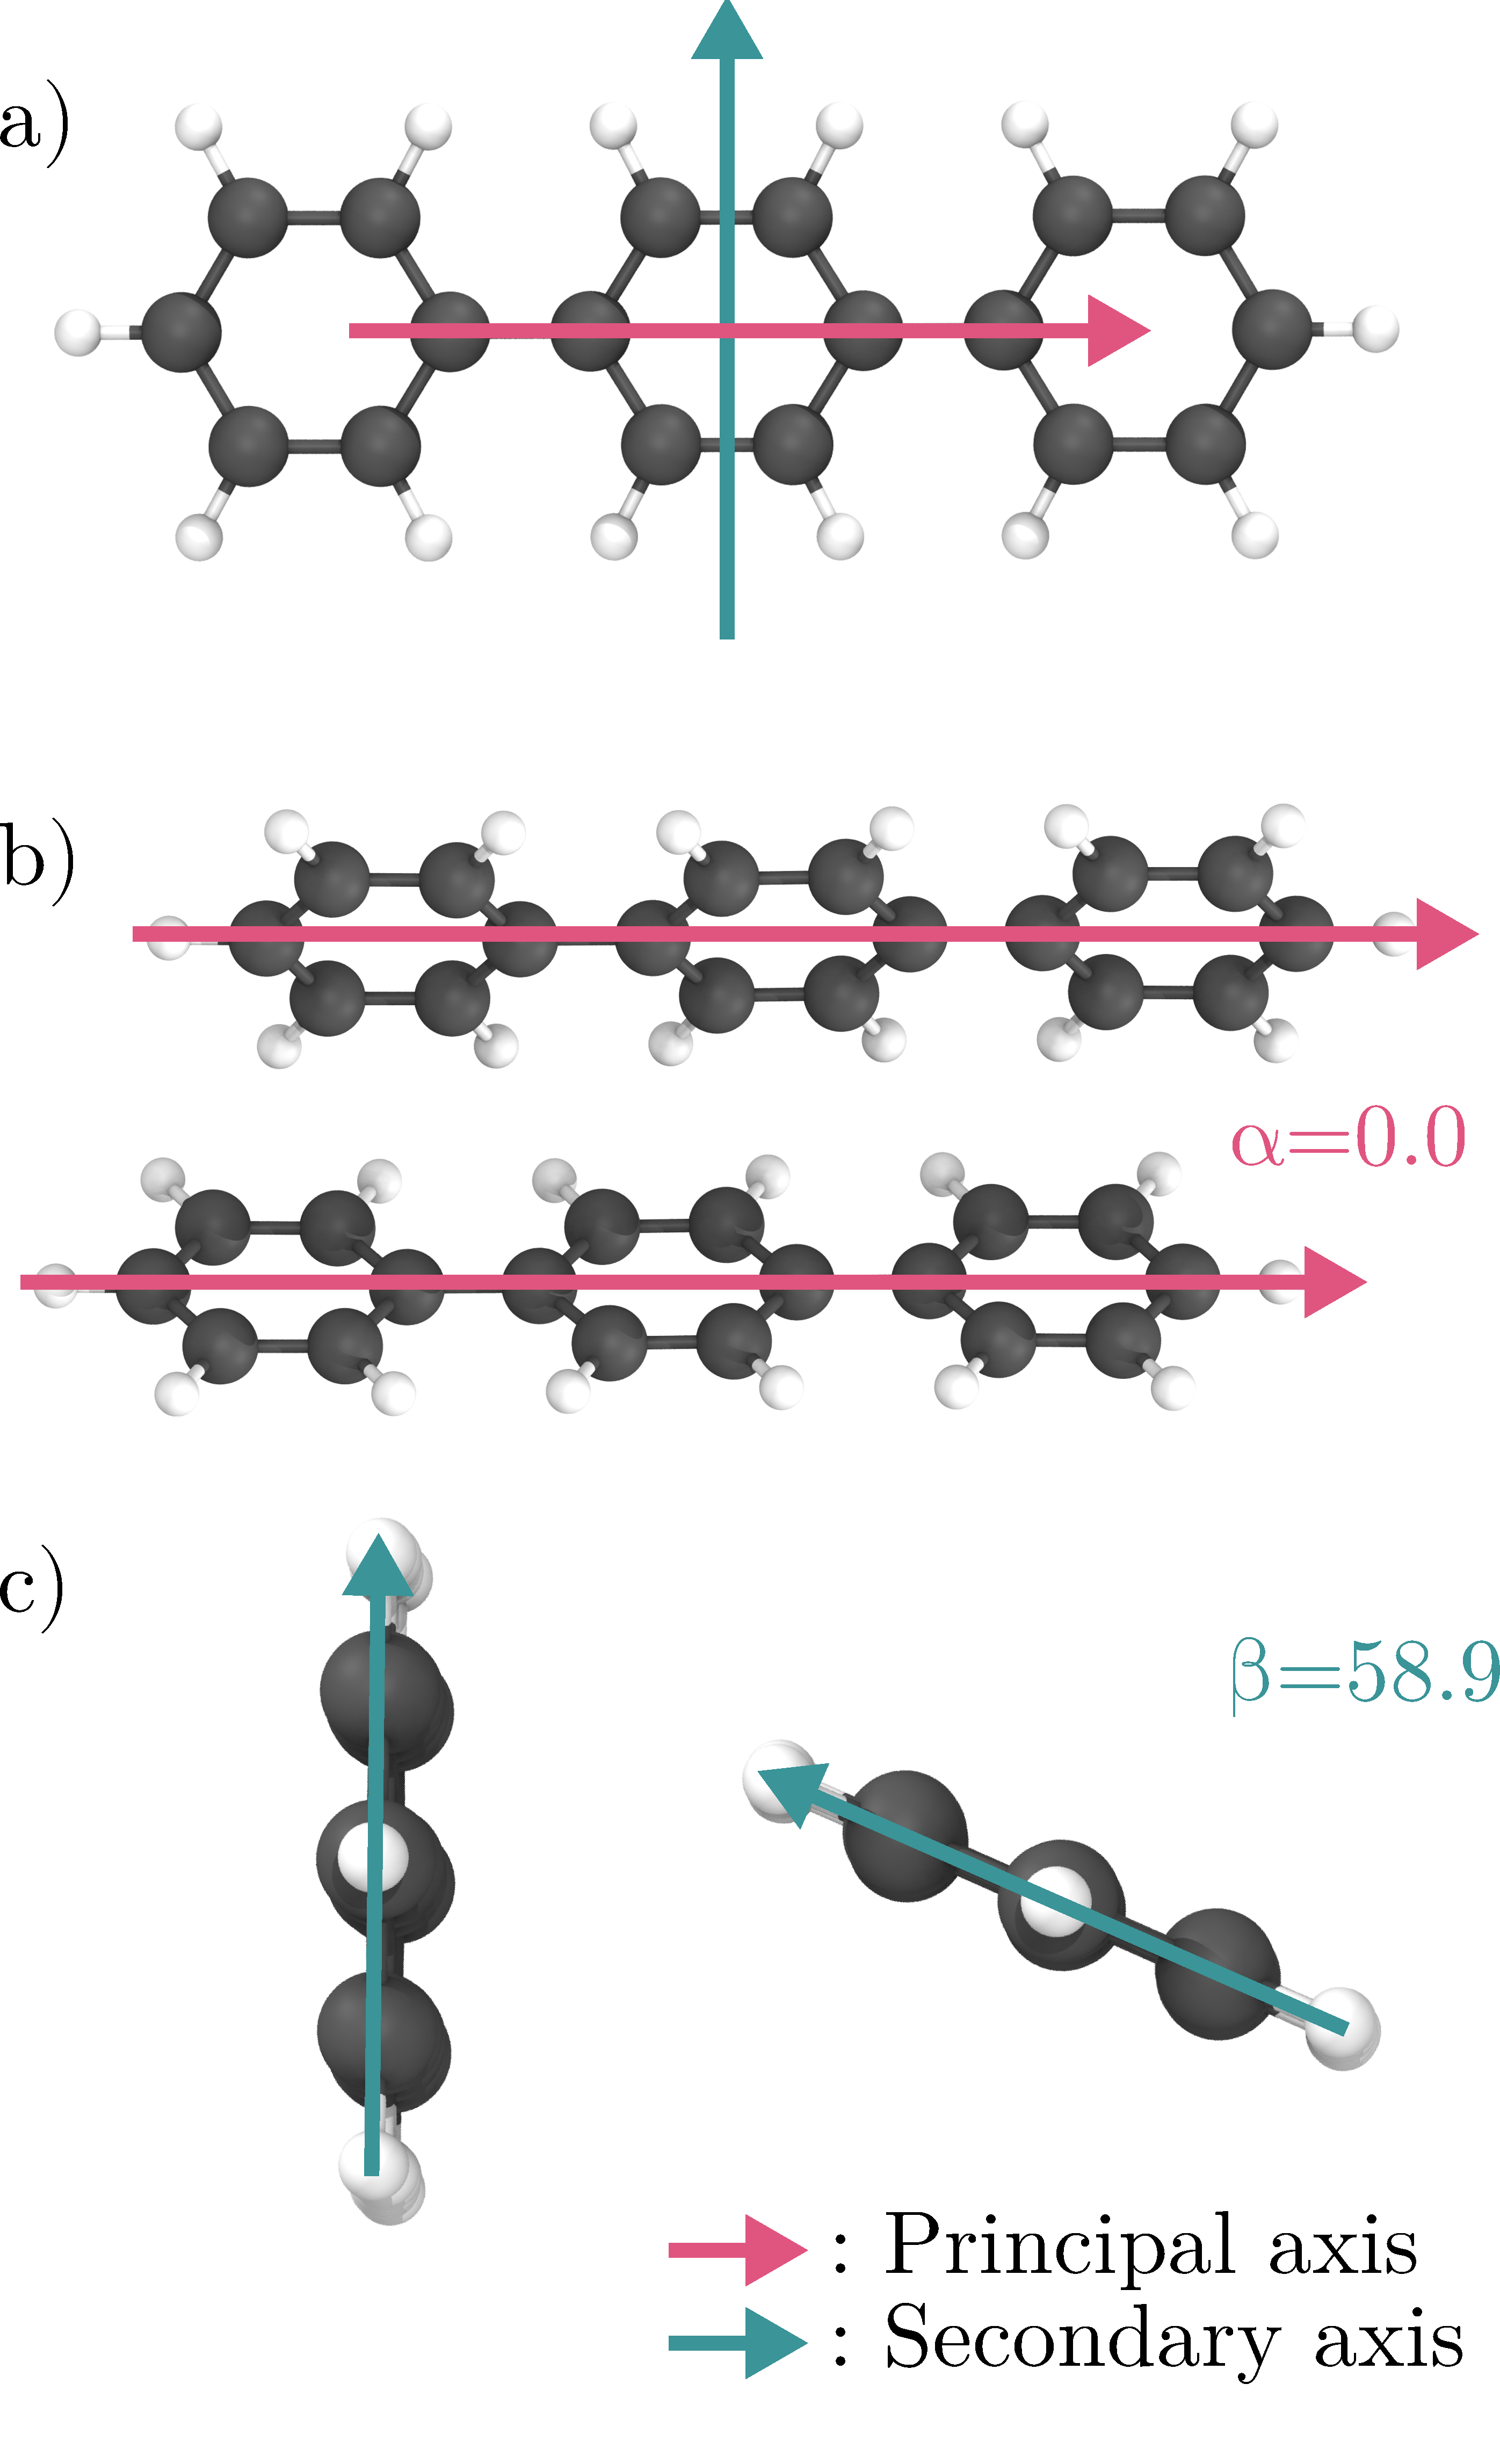
\includegraphics[width=6cm]{Chapters/7Applications/axes.pdf}
\caption{a) Principal and secondary axes on the 3P monomer b) Top view of a 3P dimer c) Side view of the same dimer.}
\label{fig:axes}
\end{figure}

All molecules have rotational symmetry about both of the axes when defined this way apart from HBT which has an inherent orientation. In the case of this molecule, we employed the scheme described in Section \ref{sec:dimer_axes} where, by exploiting the two longest interatomic distances on the averaged plane, a set of axes could be defined with consistent orientation.

To evaluate exciton couplings between dimers, the diabatisation scheme by Troisi and Arag\'o\cite{Arag2015}, as implemented in \texttt{fromage}. The transition dipole moments of the isolated monomers were compared to those in the dimer to construct a diabatic Hamiltonian, whose off-diagonal elements are the exciton couplings. The original algorithm is thoroughly described in the Supporting Information of Reference \citenum{Arag2015} and in reference \citenum{Rivera2020}. The transition dipole moments were calculated in \texttt{Gaussian}\cite{g16} using TD-$\omega$B97X-D/6-31G(d).

For QM:QM' calculations, the ONIOM scheme was used, using electrostatic embedding. The excited state level of theory was TDDFT $\omega$B97X-D/6-31G(d), with \texttt{Gaussian}, or ADC(2)/SV(P), with \texttt{Turbomole}\cite{TURBOMOLE}. The high level region was embedded in point charges from RESP calculations of DFT $\omega$B97X-D/6-31G(d) calculated in \texttt{Gaussian}. For the polar molecules HBT and $\alpha$-DCS, the electrostatic embedding was extended to include long range Coulomb interactions using the ONIOM Ewald Embedded Cluster method (OEEC).\cite{Rivera2019} The ground state level of theory was DFTB, with \texttt{DFTB+}\cite{Aradi2007}, and the embedding for the central region was done using RESP calculations with PBE/6-31G(d) calculated in \texttt{Gaussian}. Multireference SA-2-CASSCF and MS-2-CASPT2 calculations were performed with Molcas.\cite{Aquilante2016} The active spaces are reported in the Supplementary Information.

\miguel{To sample the exciton coupling of in the dimeric vibrational space of the crystal, the QM:QM' calculations were carried out on dimers to find their FC point. Then, a normal modes calculation was carried out, from which a Wigner distribution of 200 sample geometries were extracted using \texttt{Newton-X}.\cite{Crespo-Otero2012,Barbatti2014} The exciton couplings were then evaluated using the diabatisation method.}

The Huang-Rhys factors (S$_i$) for relaxation within the S$_1$ state, between S$_0$ and S$_1$ minima, were evaluated for the members of $n$P and DCS series in vacuum and crystal environment using the \texttt{DUSHIN} code.\cite{Reimers2001AMolecules} The computations were based on normal modes computed at the optimised S$_0$ and S$_1$ geometries in vacuum at the (TD-)$\omega$B97XD/6-31G(d) level and in crystal at the QM:QM' level described above. Reorganisation energies ($\lambda_i$) decomposed into normal mode contributions are related to Huang-Rhys factors as follows: 

\begin{equation}
\lambda_i = \hbar \omega_i S_i
\label{eq_hr}
\end{equation}

The Einstein\cite{Crespo-Otero2012} and Strickler-Berg\cite{SBrelation} (SB) relations were employed to evaluate radiative rates and lifetimes of selected fluorophores in solution and crystal. Einstein equation for spontaneous decay relates fluorescence rate ($k_r$) with emission energy ($\Delta E$) and oscillator strength ($f$).

\begin{equation}
k_r=\frac{2\Delta E f}{c^3}
\label{eq1}
\end{equation}

The SB relation takes into account transitions between vibronic wave functions of excited and ground states\cite{SBrelation}. According to the SB relation, the radiative rate can be evaluated as\cite{Shi2017}

\begin{equation}
k_r=0.667 [cm^2 \times s^{-1}] \frac{\nu_F^3}{\nu_A}n^2 f
\label{eq2}
\end{equation}
Where $\nu_F$ and $\nu_A$ are vertical emission and absorption energies (in $cm^{-1}$), $f$ is the oscillator strength, and $n$ is the refractive index of a solvent.

% \textcolor{blue}{(RCO: - we need here the description of the models we are using for the crystals. We also need to specify the QM:QM' methods we are considering)} 


To evaluate exciton hopping rates, the Marcus scheme was employed:
\begin{equation}
\nu_{ij}=\frac{J_{ij}^2}{\hbar}\sqrt{\frac{\pi}{\lambda k_{\text{B}}T}}\exp\bigg[-\frac{\lambda}{4k_{\text{{B}}}T}\bigg]
\label{eq:marcus}
\end{equation}
Where $J_{ij}$ is the exciton coupling between excited monomers, $\hbar$ is the reduced Planck's constant, $k_\text{B}$ is Planck's constant, $\lambda$ is the reorganisation energy computed as described above, and $T$ is room temperature of 298 K.\cite{Stehr2014,Kimura2000}
\section{Results}

\subsection{Dimeric Arrangement}
Due to the non-covalent nature of molecular crystals, photophenomena often occur locally\cite{Arag2015} and can be understood on the scale of the nearest neighbour molecules. In particular, the conformational features of the dimer arrangements resulting from the packing of the crystal can elucidate the pairwise interactions affecting the excited states in the crystal.

The packing motifs of these materials are diverse and smoothly varying, making them challenging to classify. However certain patterns have been identified to occur frequently, and we use these as reference points.\cite{Desiraju1989,Campbell2017} In particular, herringbone crystals pack in an alternating edge-to-face arrangement, while sheet crystals have all molecules sharing the same orientation arranged in regular layers. These two motifs are represented in Figure \ref{fig:packing}. \miguel{For the sake of clarity, in this chapter, we employ the terms like \textit{herringbone} and \textit{sheet} to refer to the overall crystal packing, and ones like \textit{edge-to-face} or \textit{face-to-face} to denote specific dimer arrangements.}

\miguel{Table \ref{tab:molecules} summarises the principal data relating to the packing and emission of all systems. We immediately note the prevalence of H dimers arising from the herringbone and sheet packing patterns, which result in significant QEF values, contradicting Kasha's exciton model.\cite{Kasha1965} The intermolecular processes in these materials therefore must go beyond point-dipole approximations.}

\begin{figure}
\centering12
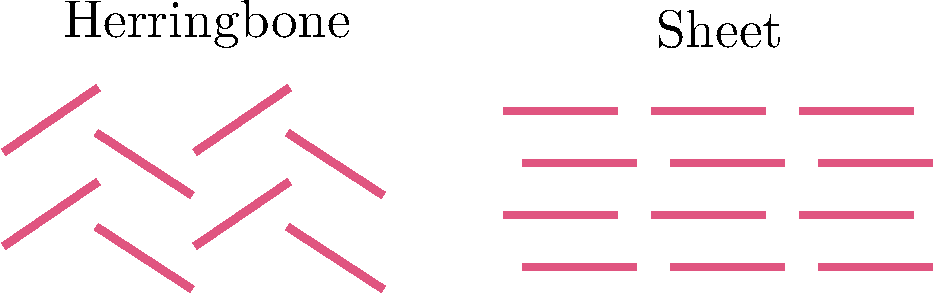
\includegraphics[width=7cm]{Chapters/7Applications/packings.pdf}
\caption{Illustration of two archetypal packing motifs in molecular crystals.}
\label{fig:packing}
\end{figure}

The significant dimers of the crystals in consideration were processed in \texttt{fromage} to extract their characteristic angles. The overall crystal packing was found to be split between the series of molecules. The DCS series primarily forms sheets, while the other crystals have a clear bias towards herringbone motifs. The principal axis angles in face-to-face dimers of sheet crystals are almost always 0\degree{} due to the translational symmetry between layers. In contrast, herringbone crystals usually have nearly parallel principal axes and a large array of secondary axis angles. Indeed the tilt between herringbone layers is strongly dependent on the morphology of the constituent fragments.

\begin{figure}
\centering
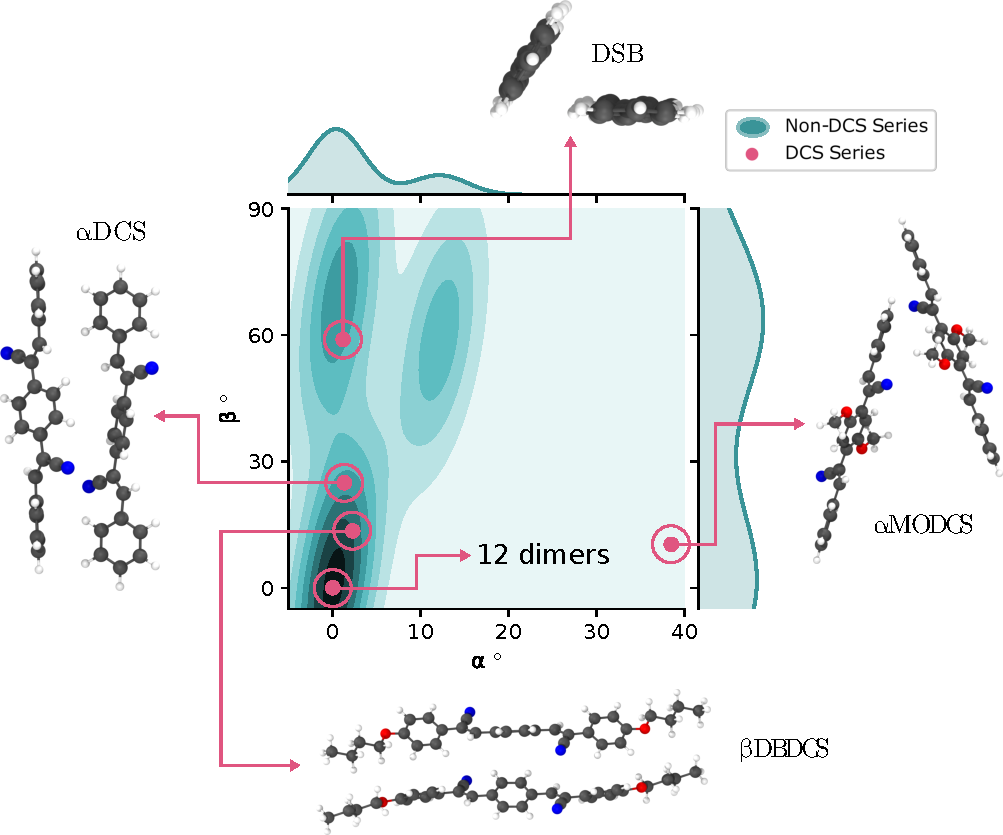
\includegraphics[width=9cm]{Chapters/7Applications/angles.pdf}
\caption{Distribution of the dimeric arrangements in the DCS series (14 dimers) and the rest of the crystals (14 dimers). The angle between principal axes is plotted against the angle of the secondary axes. Almost all DCS series dimers are perfectly parallel, the exceptions are shown.}
\label{fig:angles}
\end{figure}


The angle values for non-DCS series crystals are represented as a density map in Figure \ref{fig:angles}. The herringbone and sheet families of crystals can be spotted by their characteristic densities centred around (0\degree{},0\degree{}) and (60\degree{},15\degree{}) respectively. Herringbone crystals also contribute to the density at (0\degree{},0\degree{}), given that they are made up not only of edge-to-face dimers but also of face-to-face ones. Furthermore, there is more configurational variety in edge-to-face dimers, as evidenced by the wide spread of $beta$ angles. The island of dimers of $\alpha$ angles larger than 10\degree{} is due only to one 4PV dimer and two HBT dimers. This slight departure from ideal herringbone packing is known in 4PV\cite{VanHutten1999}, where the unit cell includes six molecules instead of two. HBT displays slightly misaligned head-to-tail dimers indicating that each layer of the material in the principal axis direction has an alternating orientation.

The DCS series dimers are represented as a points on the same plot. All of the points were found at the (0\degree{},0\degree{}) position, except for four outliers. DSB has a dimer at (1.2\degree{},58.9\degree{}), which is near the centre of the dense shaded area. This confirms the nature of DSB as a herringbone crystal, which becomes a sheet crystal only following substitutions. $\alpha$-DCS and $\beta$-DBDCS have dimers at (1.3\degree{},24.9\degree{}) and (2.3\degree{},13.5\degree{}) respectively, which break the translational symmetry due to the freedom of rotation of their central aromatic ring. $\alpha$-MODCS has a point at (38.5\degree{},10.3\degree{}), which is far away from any other considered dimer. The packing of this crystal does not match any of the common packing classifications.

\subsection{Exciton Coupling}
The values of the exciton couplings of the molecules under scrutiny, evaluated at their Frank-Condon region, are a result of structural and chemical features of the dimers formed upon aggregation. We therefore wish to highlight any possible correlations between the packing patterns described above, and the exciton states within the crystal. These states are liable to cause delocalised excitation phenomena, discouraging emission.

We first examine the dependence of the couplings on the distance between constituent fragments of the dimer. Figure \ref{fig:dist} shows the exciton coupling of each dimer of the crystal structures with respect to the centroid-to-centroid distance of said dimer. We observe a clear monotonic downward trend for dimers belonging to every crystal except for HBT. This trend is in line with the limiting behaviour where fragments become non interacting at infinite distances and the coupling should therefore tend to zero. In the middle to long range, the electrostatic interaction between the two fragments approaches a $1/r$ shape where $r$ is the distance between the centres of mass of each electron could. Figure \ref{fig:dist} does not have the sufficient resolution to suggest an inverse law as opposed to other monotonically decreasing functions. However, we can observe that dimers from different series have similar exciton coupling given similar centroid-to-centroid distance \miguel{within a range of 50 meV. This is a surprising result because of the inadequacy of centroid distance as a measure of correlation of neighbouring excited states, ignoring the shape of the molecular wavefunctions altogether.}

\begin{figure} [h!]
\centering
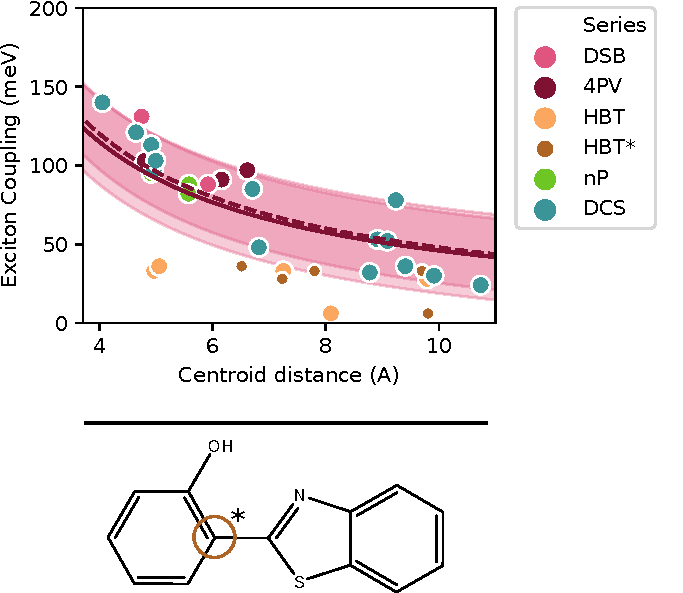
\includegraphics[width=8cm]{Chapters/7Applications/dist_coupling.pdf}
\caption{(top) Exciton coupling (J) as a function of the centroid-to-centroid distance of the constituent monomers of each dimer. The values of every dimer are fitted to an inverse law $f(r) = a/r$ \textit{via} least squares. The resulting function, with $a=459$ is plotted in pink and has a standard deviation of 27, represented by the shaded area. A dashed line represents the same fit but using an aromatic carbon (bottom) as a reference for the distance calculation, denoted HBT*. In this case, $a=480$ and the standard deviation is 23.}
\label{fig:dist}
\end{figure}

HBT constitutes a striking exception, where all of the nearest neighbour dimers have exciton coupling values between 20 and 40 meV. In particular, the two closest dimers, with centroid distances close to 5 \AA{}, are about 60 meV below the fit line. The transition densities of these dimers, compared with the monomer transition density are depicted in Figure \ref{fig:hbt_dens}. The excitation of the isolated molecule is mainly localised in the proton transfer moiety, breaking the apparent symmetry of the two constituent rings. Both closest dimer arrangements are aligned in centroid but opposite oriented, effectively distancing the excitation densities. This effect is less pronounced in other molecules because they are all symmetric in orientation of their long axis. By measuring the distance between HBT molecules with an aromatic carbon as a reference point, the exciton coupling values adopt a clearer downward trend, albeit shifted lower than for the other series.

\begin{figure}
\centering
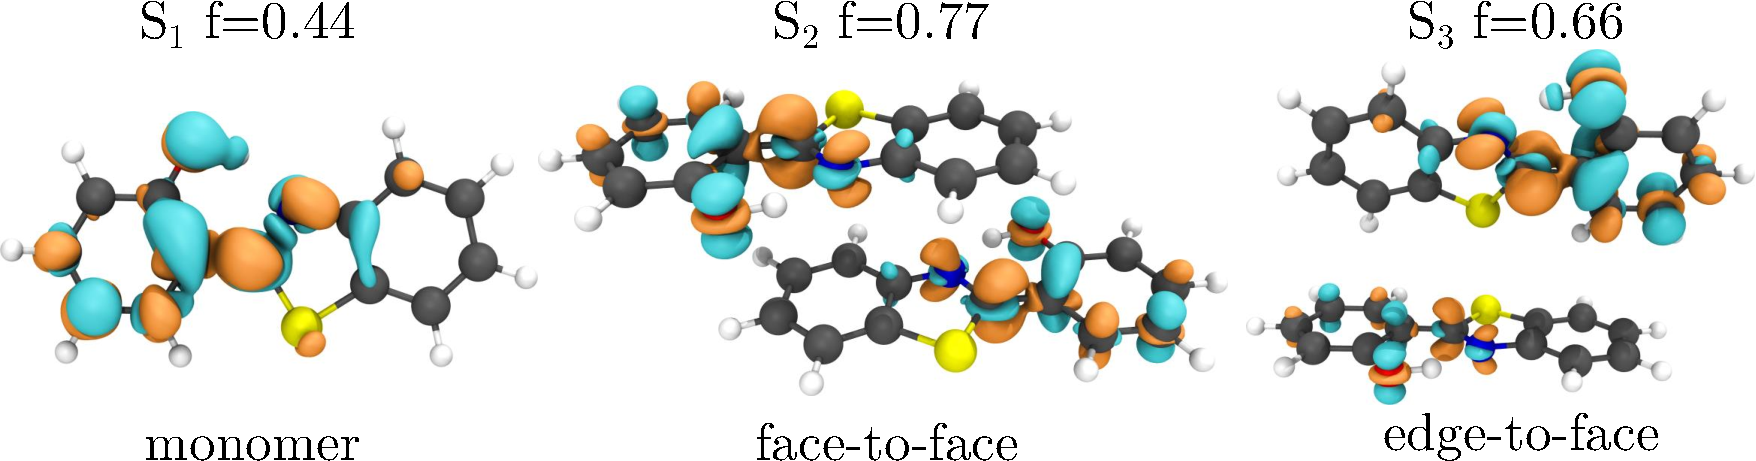
\includegraphics[width=9cm]{Chapters/7Applications/hbt_dens.pdf}
\caption{Transition densities of the bright states of HBT in monomer form and both dimers of least centroid-to-centroid distance. Upon excitation, the density is reorganised from the blue to the orange areas.}
\label{fig:hbt_dens}
\end{figure}

Excluding HBT, the dimers are roughly split into two group, those below 7 \AA{} in separation, with couplings ranging from 82 to 140 meV and those above 7 \AA{} with couplings from 24 to 64 meV. Those in the former group are overall above the $a/r$ trend line, and those of the latter below. This may be explained by the added proportion of exciton coupling resulting from exchange in the strong coupling regime. Ref. \citenum{Fornari2017} found that when Coulombic coupling exceeds 70 meV in organic semiconductor materials and light-harvesting complexes, the exchange portion of the coupling always shares a sign with its electrostatic counterpart, thus increasing the total coupling. This is consistent with the deviation of the limiting behaviour of the total coupling from a Coulombic inverse law.

\begin{figure}
\centering
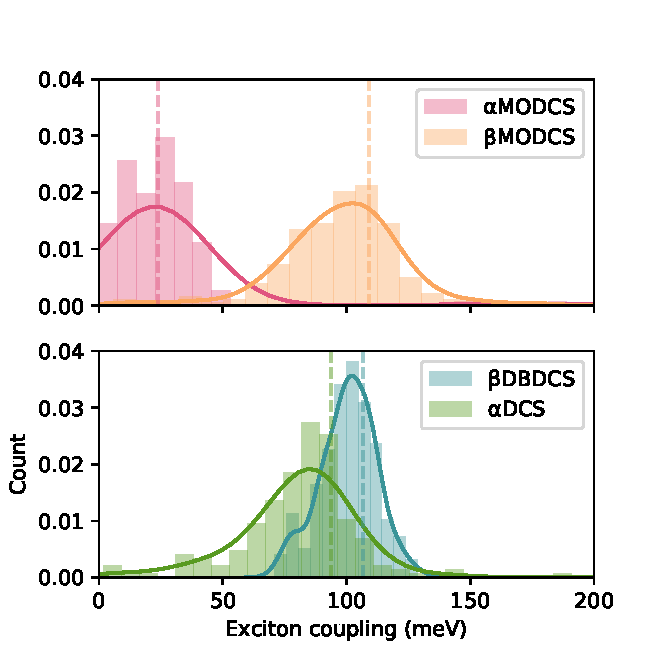
\includegraphics[width=8cm]{Chapters/7Applications/hist.pdf}
\caption{Exciton coupling values of irregularly packed DSB dimers, sampled from their vibrational phase space.}
\label{fig:hist}
\end{figure}


\begin{table*}
\scalebox{0.7}{
\begin{tabular}{@{}lccccccccccc@{}}

%\begin{tabular}{@{}llllllllllll@{}}
\toprule
\multirow{2}{*}{Crystal}    & \multirow{2}{*}{Series}  & \multirow{2}{*}{$V_i$} & \multirow{2}{*}{J (meV)$^a$} &   \multirow{2}{*}{Packing$^b$}  & \multirow{2}{*}{H dimer \%$^c$} & \multicolumn{3}{c}{Calculated absorption}& \multirow{2}{*}{Exp. absorption} & \multirow{2}{*}{$\Phi_f$}\\
& & & & & & Monomer & Dimer S$_1$ & Dimer S$_2$ &  & \\\midrule

%& E S1 dimer & E S2 dimer &   \\ 
DSB        & - & 1.41         & 131       & HB     & 100      & 3.60      & 3.47       & 3.65       & 3.48$^d$\cite{Shi2017}                        & 0.78          \\
4PV        & - & 1.42         & 103       & HB    & 100       & 3.10      & 2.98       & 3.19       &                -             & -           \\
HBT        & -     & 1.43         & 36       & HB & 83 & 3.98      & 3.94       & 4.00       & 3.65$^e$\cite{Lee2013}                  &  0.77$^g$\cite{hbt_exp}  \\
3P         & $n$P      & 1.37         & 98        & HB    & 100       & 4.36      & 4.24       & 4.43       & 4.51$^d$\cite{Pavlopoulos1974}                         & 0.67\cite{Katoh2009}          \\
4P         & $n$P      & 1.39         & 99        & HB    & 100       & 4.16      & 4.05       & 4.23       & 4.13$^d$\cite{Pavlopoulos1974}                         & -           \\
6P         & $n$P      & 2.27          & 95        & HB    & 100       & 3.75      & 3.63       & 3.82       &                  -           & 0.30$^h$\cite{6P_qy}  \\
$\alpha$-DCS     & DCS     & 1.41         & 97        & S      & 100   & 3.74      & 3.60       & 3.80       & 3.61$^f$\cite{Shi2017} & 0.90\\
$\alpha$-DBDCS   & DCS     & 1.49         & 53        & S  & 100   & 3.33      & 3.19       & 3.30       & 3.34$^f$\cite{Shi2017}                         & 0.62          \\
$\beta$-DBDCS   & DCS     & 1.53         & 113       & S  & 100 &  3.30      & 3.17       & 3.34       & 3.19$^f$\cite{Shi2017}                        & 0.84          \\
$\alpha$-MODCS   & DCS     & 1.42         & 32        & -  & 50 & 3.66      & 3.64       & 3.69       & 3.45$^e$\cite{Shi2017}                        & 0.66          \\
$\beta$-MODCS   & DCS     & 1.39         & 140       & S   & 100  & 3.06      & 2.86       & 3.13       & 2.95 3.60$^f$\cite{Shi2017}                   & 0.73          \\
$\alpha$-MODBDCS & DCS     & 1.44         & 103       & S   & 100  & 3.27      & 3.22       & 3.29       & 3.43 3.84$^f$\cite{Shi2017}                   & 0.42          \\
$\beta$-MODBDCS & DCS     & 1.43         & 121       & S   & 100  & 2.80      & 2.68       & 2.84       & 2.87 3.40$^f$\cite{Shi2017}                   & 0.46          \\ \bottomrule
\end{tabular}
}
\caption{Photoactive molecular crystals considered. $\Phi_f$: fluorescence quantum yield in crystal, $V_i$: steric volume index. $^a$ Largest dimeric exciton coupling in the crystal, $^b$ Herringbone (HB), Sheet (S) or other (-), $^c$ fraction of H (not J) dimers in the crystal, $^d$ tetrahydro-2-metehylfuran solvent, $^e$ cyclohexane solvent, $^f$ chloroform solvent, $^g$ powder, $^h$ film.}
\label{tab:molecules}

\end{table*}

Moreover, we observe a clear linear dependence of the exciton coupling on the dimeric S$_2$\textendash{}S$_1$ gap, depicted in Figure \ref{fig:half}. This can be understood by definition, in the limit of linear resonant molecules.\cite{Spano2016} The S$_2$ and S$_1$ states of the dimer are composed of superpositions of equal and symmetric S$_1$ adiabatic monomer states, and the splitting is only due to the exciton coupling. The remarkable agreement with the fit line implies a strong degree symmetry of the two constituent molecular wavefunctions, characteristic of the herringbone and sheet packing characterised in the previous section.

\begin{figure}
\centering
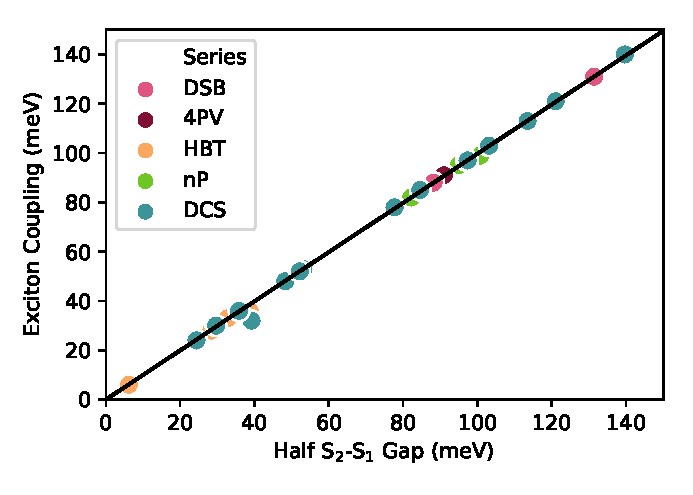
\includegraphics[width=8cm]{Chapters/7Applications/half_gap.pdf}
\caption{Exciton coupling as a function of half of the S$_2$\textendash{}S$_1$ energy gap. The linear trend line, obtained \textit{via} least squares, is $f(x) = 0.997x$}
\label{fig:half}
\end{figure}

We would also like to probe for any link between the geometric dimer arrangements and exciton coupling values. We sample the vibrational phase space of four dimers of the DCS series: two close to sheet-like packing crystals ($\alpha$-DCS and $\beta$-DBDCS), one perfect sheet crystal ($\beta$-MODCS) and the unclassified outlier $\alpha$-MODCS. The results are shown in Figure \ref{fig:hist}.

We can observe a grouping of vibrational ground state exciton coupling values of 94, 107, and 109 meV for the face-to-face dimers (respectively $\alpha$-DCS, $\beta$-DBDCS, and $\beta$-MODCS), well away from the value of 24 meV for $\alpha$-MODCS. When compared with the corresponding centroid-to-centroid distances\textemdash{}4.95, 4.64, 4.91, and 8.78 \AA\textemdash{}we observe the correlation with interatomic distance mentioned previously. $\beta$-DBDCS shares a similar interatomic distance than $\alpha$-DCS and $\beta$-MODCS, despite its additional buthoxy chains which lengthen the backbone. We can therefore link crystals of this series with similar packing motifs, to a similar interatomic distance, and a similar Franck-Condon geometry exciton coupling.

The broadness of the peaks offers an insight on how the dimers' thermal motions can influence their exciton couplings. From narrowest to broadest, the standard deviations are 11 meV for $\beta$-DBDCS, 27 meV for $\beta$-MODCS, 35 meV for $\alpha$-MODCS, and 51 meV for $\alpha$-DCS. $\alpha$-MODCS and $\beta$-MODCS are the two systems with closest molecular structure, and also the most similar standard deviation in exciton coupling values, despite their radical packing difference. $\beta$-DBDCS has a spread of about a third that of $\beta$-MODCS, and a fifth that of $\alpha$-DCS despite them all displaying sheet-like packing. To summarise, in these systems, since exciton coupling is a many-body property, its value at fixed geometry depends on intermolecular structure properties. However the thermal fluctuation in exciton coupling depends on the vibrational phase space of the crystal dimers, which in this case is determined predominantly by molecular structural factors, not the dimer arrangement. \miguel{Crystal-scale vibrations are not probed by this model, and we cannot comment on the importance of exciton-phonon effects.}

\subsection{Excited-state Relaxation by Series}
Whilst geometrical considerations are easily transferable from series to series, their nonradiative decay mechanisms are usually considered to be highly system-specific since they are directly dependent on the molecular conformations available to the molecule in question. In this section, we illustrate this point by investigating the excited-state decay processes of chemically diverse molecules.

\textbf{HBT}

2-(2'-hydroxyphenyl)-benzothiazole (HBT) displays SLE upon its aggregation to herringbone single crystal\cite{hbt_derivatives1} and liquid crystal phases.\cite{hbt_lc} While HBT has low QEF in organic solvents;\cite{hbt_exp,hbt_solvents} in the aggregate phase (THF/water solution, 1:9, v/v) and in powder, the yields are 0.09 and 0.77, respectively.\cite{hbt_exp} For this reason, HBT-derivatives are proposed as materials for organic light-emitting diodes (OLEDs) and fluorescent probes.

The underlying excited state relaxation mechanism of HBT-based systems includes excited state intramolecular proton transfer (ESIPT) in vacuum, solution,\cite{Mario_HBT, HBT_multiplespawning} and crystal \cite{hbt_esipt0,hbt_esipt}. In vacuum and solution, the process is known to be a four-step photophysical cycle enabled by an intramolecular hydrogen-bonding. It consists of a photon absorption, excited-state proton transfer, torsional motion, and the ground-state proton back-transfer\cite{Mario_HBT,hbt_esipt}. The process is characterised by large reorganisation energies dependent on the nature of the solvent.\cite{Mario_HBT,hbt_esipt}

Reorganisation energy can be used to deduce the most efficient relaxation pathways within the excited state PES. We optimised the S$_0$ and S$_1$ states of keto and enol forms of HBT in solution and in the solid state. Following the excitation to the S$_1$ state of the enol form, there are two possible pathways: relaxation to the S$_1$ minimum of the enol form, and ESIPT yielding cis-keto form in the $S_1$ state. The reorganisation energies in the S$_1$ state released during these processes are 0.28 eV for the former and 0.38 eV for the latter in cyclohexane and 0.27 eV and 0.39 eV respectively in the solid state. Thus, the ESIPT process is energetically encouraged.

Additionally, in crystal, the enol emission energy has a 0.54 eV difference with the enol absorption energy and 0.27 eV with the keto absorption energy. In contrast, the keto emission has differences of 1.27 eV and 0.56 eV respectively. This indicates reabsorption is much likelier to occur with light emitted from the enol form, thus quenching this radiative decay channel. Indeed fluorescence experiments have observed emission from both the enol and keto forms in solution solution\cite{hbt_esipt2} and only from the latter in crystal,\cite{HBT_laser} where the packing is closer and the chances for reabsorption greater, only from the latter.

We now attempt to rationalise the SLE mechanism of HBT \textit{via} the lens of the Restricted Access to Conical Intersections (RACI) model outlined by Blancafort \textit{et al.} in References \citenum{Li2013} and \citenum{Blancafort2018}. This framework compares the energy of the MECI energy to the vertical absorption in order to determine the viability of internal conversion through a conical intersection. Our previous work has already proven the efficacy of this method for aromatic ESIPT materials, which indicates that other nonradiative mechanisms can be put aside for now.\cite{Dommett2017a,Dommett2019} We used similar ONIOM Ewald Embedded QM:QM' Cluster methods (OEEC), to optimise critical regions of the solid state potential energy surface. We used the Ewald embedding scheme to account for the long-range electrostatic interactions of the material, which can be important in polar crystals. We chose the $\omega$B97X-D functional since it has reproduced accurate ESIPT optimised geometries in the past, and predicts a QM:QM' absorption energy of 4.20 eV, as compared to the experimental value of 3.65 eV. The results are depicted in Figure \ref{fig:hbt_e}.

The conical intersection which involves only a rotation of the oxygenated aryl bond is the S$_1$\textendash{}S$_0$ MECI in solution, but becomes very unstable due to the steric hindrance of the nearest neighbour molecules upon crystallisation. The S$_1$\textendash{}S$_0$ MECI in crystal additionally involves the pyramidalisation of one of the molecular backbone carbons, thus reaching a distorted but spatially compatible geometry within the close packed environment. However due to this distortion, the crystal MECI remains unstable, surpassing the absorption energy by 1.9 eV. If we use MS-2-CASPT2(12,12)/aug-cc-pVDZ as the excited state method instead, using the geometries optimised in TDDFT, the results are similar, with an absorption of 3.88 eV\textemdash{}now only 0.23 eV above the experimental value\textemdash{}and a MECI 2.05 eV above absorption. In this case, the $S_1$\textendash{}$S_0$ gap at the MECI geometry is 0.36 eV. Further scanning of the CASPT2 PES would help narrow this gap, but would be unlikely to reduce the energy by up to 2.05 eV.

Upon crystallisation, the S$_1$\textendash{}S$_0$ MECI becomes inaccessible for a molecule excited at FC point. This blocks the principal nonradiative decay channel, and explains the 8 to 9 fold rise in QEF from measurements in organic solvent and in powder samples. In this case, alternative nonradiative decay channels are not important enough in the crystal to prevent the formidable 0.77 efficiency.

\begin{figure}
\centering
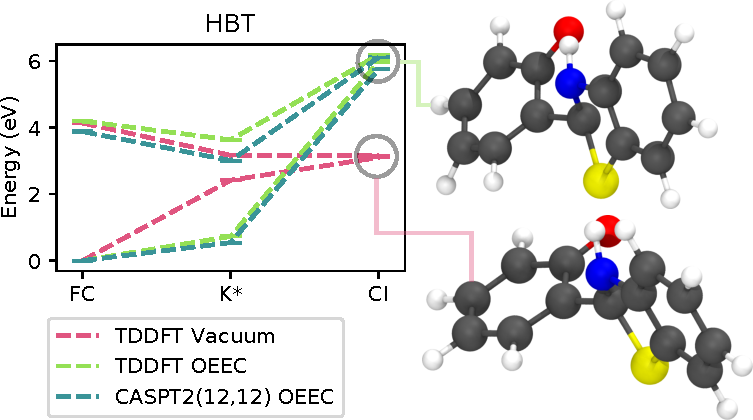
\includegraphics[width=8cm]{Chapters/7Applications/HBT_energy.pdf}
\caption{HBT energy at critical points of its excited state potential energy surface. The vacuum calculation used TD-$\omega$B97X-D/6-31G(d) and the crystal calculation TD-$\omega$B97X-D/6-31G(d):DFTB.}
\label{fig:hbt_e}
\end{figure}


\textbf{$n$P}

p-Hexaphenylene (6P) has been employed as a building block of photonic nanofibers,\cite{6P_fibers, 6P_fibers2} and as a material for nanolasers,\cite{6P_nanolaser, 6P_nanolaser2} exploiting its amplified spontaneous emission,\cite{6P_ASE} thanks to its fluorescence and structural characteristics favourable for growing well-defined molecular architectures. 

6P has an experimental fluorescence quantum yield of 0.85 in solution and 0.30 in crystal,\cite{6P_qy} whereas the much smaller 3P has a yield of 0.82 in solution\cite{Mukundam} and 0.67 in crystal.\cite{Katoh2009} We would like to rationalise this difference, also considering the intermediate case of 4P. In contrast with HBT, these systems are emissive in vacuum, meaning that their excited state process in vacuum is not dominated by nonradiative deactivation.

% Its reported significant value of experimental fluorescence quantum yield ($\Phi_f$=0.30)\cite{6P_qy} could suggests important nonradiative mechanisms and photon reabsorption in the film. The smaller p-terphenylene (3P) has a more efficient fluorescence in single crystal ($\Phi_f$ = 0.67), powder samples ($\Phi_f$ = 0.80) \cite{Katoh2009}, and in cyclohexane solution ($\Phi_f$ = 0.82).\cite{Mukundam}

We optimised the structures of the emitting $\pi\pi^*$ states of 3P, 4P, and 6P, applying TD-$\omega$B97X-D in cyclohexane solvent using PCM and in the crystal phase with the QM/QM' cluster method at the TD-$\omega$B97X-D/DFTB level including one molecule in the QM region. From the computed S$_1$ energies and oscillator strengths (Table \ref{tab:Rates}), several interesting trends can be observed.

As the length of the chain increases from three to four and four to five, the emission energy decreases. The trend is similar in solution and in crystal where in the former, the emission energy decreases by 0.20 eV from 3P to 4P and by 0.17 eV from 4P to 6P, and in the latter the differences are 0.21 eV and 0.28 eV.

We can relate this phenomenon to the degree of delocalisation of the transition density in the different molecular structures. As can be seen in Figure \ref{fig:nP_delocalisation}, in the case of 3P, the S$_1$ transition density is mostly localised on the central phenyl ring and surrounding C\textendash{}C bonds, while in the case of 4P and 6P, it is localised on two central phenyl rings and surrounding C\textendash{}C bonds. This delocalisation destabilises the HOMO and stabilises the LUMO, which contributes to narrowing the S$_1$\textendash{}S$_0$ energy gap. This could also explain the increases in oscillator strength by 0.54 and 0.90 in solution, and 0.55 and 1.12 in crystal, where a more diffuse transition is correlated with a greater overlap between initial and final wavefunctions and a greater transition dipole moment.

In comparison with the solution, the crystal environment raises the emission energy by 0.1 eV and lowers the oscillator strength by 0.2 for 3P and 4P. These effects are, however, negligible for 6P.

\begin{figure}
\centering
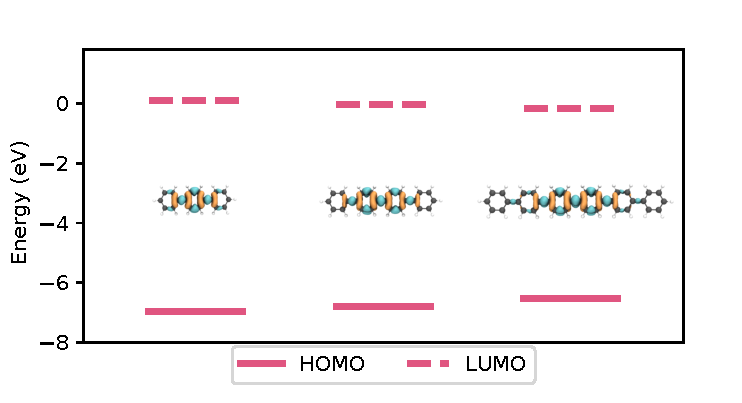
\includegraphics[width=6cm]{Chapters/7Applications/nP_delocalisation.pdf}
\caption{The energies of HOMO and LUMO orbitals of 3P, 4P, and 6P in the crystal computed at the TD-$\omega$B97X-D/6-31G(d) level. The S$_1$ transition densities are represented as well.}
\label{fig:nP_delocalisation}
\end{figure}


The emission rates, $k_r$, computed applying Einstein relation in solution and crystal and applying the SB relation in solution, increase with backbone length. This is due to the large increase of oscillator strength relative to the decrease in emission energy. The $k_r$ values in solution and in crystal are very similar throughout the series due to competing effects of crystallisation increasing the emission energy and decreasing the oscillator strength for 3P and 4P.

The rates in solution obtained based on the SB relation are about twice as large as the values obtained from Einstein relation. This is due to the transitions between vibronic wave functions of the excited and ground states, which the Einstein relation neglects.

\begin{table*}
\scalebox{0.8}{
\begin{tabular}{@{}lcccccccccccc@{}}
\toprule
\multirow{2}{*}{Molecule}   & \multirow{2}{*}{ $E(S_1)^{\text{sol}}$} & \multirow{2}{*}{ $f^{\text{sol}}$ } & \multirow{2}{*}{$k_r^{\text{Ein,sol}}$} & \multirow{2}{*}{$k_r^{\text{SB,sol}}$} & \multirow{2}{*}{$\Phi_f^{\text{sol}}$} & \multirow{2}{*}{$\lambda^{\text{vac}}$} & \multirow{2}{*}{ $E(S_1)^{\text{cr}}$} & \multirow{2}{*}{ $f^{\text{cr}}$} & \multirow{2}{*}{$k_r^{\text{cr}}$} & \multirow{2}{*}{$\Phi_f^{\text{cr}}$} & \multirow{2}{*}{$\lambda^{\text{\text{cr}}}$} \\
\\
\midrule
3P        & 3.69 & 1.37 & 0.81 & 1.24 &  0.82\cite{Mukundam} & 0.51 & 3.83 & 1.19 & 0.76 & 0.80$^a$\cite{Katoh2009} , 0.67$^b$\cite{Katoh2009} &  0.35\\
4P        & 3.49 & 1.91 & 1.01 & 1.54 &     -                &0.54 & 3.62 & 1.74 & 0.99 &   -                                                         & 0.37\\
6P        & 3.32 & 2.81 & 1.35 & 2.17 &     -                & 0.49 & 3.34 & 2.86 & 1.38 & 0.30$^d$                                                    & 0.29\\
\bottomrule
\end{tabular}
}

\caption{Computed S$_1$ energies in eV ($E(S_1)$) with corresponding oscillator strength ($f$), radiative rates calculated with the Einstein relation and SB formula in ns$^{-1}$ ($k_r^{\text{Ein}}$, $k_r^{\text{SB}}$), experimental luminescent efficiency ($\Phi_f$), and reorganisation energies in eV ($\lambda$) for the $n$P series. The superscripts indicate the medium, where "sol" is cyclohexane solvent, "vac" is vacuum, and "cr" is crystal. $^a$Powder samples. $^b$ Single crystal.}

\label{tab:Rates}
\end{table*}

%Significant values of exciton couplings in the case of all three systems ($J$ $\sim$ 0.1 eV) suggest that emission rates could be affected by excitonic effects. 

% Optimisation of the S$_1$ state of a $\pi$-stacked 3P dimer shows that both S$_1$ and S$_2$ states at the S$_1$ geometry are bright ($f(S_1)=0.60$), which indicates that emission in crystal cannot be explained based on the model of monomer embedded in crystal environment.
%\textcolor{blue}{(RCO: the couplings are very similar, the differences should be related with the nonradiative pathways. Solution, getting the conicals..)}

The decrease in QEF of 6P with respect to 3P is not explained by the behaviour of radiative rates which instead increase with chain length. This raises the question of the importance of nonradiative relaxation pathways in this series. \mmiguel{We first examine a rationalisation based on conical intersections, as this was a determining factor for HBT.}


The S$_1$\textendash{}S$_0$ minimum energy crossing points were optimised at the ADC(2)/def-SV(P) level in vacuum and crystal for 3P, 4P, and 6P. TD-$\omega$B97X-D/6-31G(d) was also attempted but electronic convergence problems arose due to the highly distorted conformations involved. Previous studies indicate that ADC(2) can represent accurate S$_1$\textendash{}S$_0$ crossing topologies in organic chromophores despite being a single reference method.\cite{Tuna2015}

The optimised vacuum S$_1$\textendash{}S$_0$ MECI geometries of 3P and 4P, represented in Figure \ref{fig:nP_pathways}, correspond to ring puckering conical intersections with puckered phenyl rings on which the S$_1$ transition densities are localised. The central phenyl ring at the MECI geometry of 3P in vacuum is a prefulvene kind of conical intersection,\cite{Olivucci} characterised by a half-boat structure with the $C_s$ symmetry.
%It has previously been identified as a global intersection space minimum of benzene in vacuum.\cite{Blancafort_benzene,Blancafort_benzene2}
The puckering of the central ring is accompanied by flapping motion of peripheral phenyl rings, resulting in a highly distorted structure with one phenyl ring roughly perpendicular to the puckered ring.

However, in the crystal, ring-puckering and flapping motions are partially hindered due to the tight packing. As a result, the crystal S$_1$\textendash{}S$_0$ MECI geometry has a different identity, featuring a pronounced puckering of one C atom of the central ring and substantial out-of-plane distortion of H atom attached to it. The rest of the molecule remains in plane. This conical intersection corresponds to another point at the prefulvene CI seam.

Similarly, the S$_1$\textendash{}S$_0$ MECI structure of 4P in vacuum corresponds to a puckered half-boat structure of one of the central rings, while the other one, on which transition density is also localised at the S$_1$ minimum, displays slight out-of-plane distortion.

The 4P S$_1$\textendash{}S$_0$ MECI structure in crystal phase is similar to the one obtained for 3P. The restriction of large out-of-plane motions can be explained by the herringbone packing of these crystals. Figure \ref{fig:angles} shows how the two prevalent packing motifs\textemdash{}herringbone and sheet\textemdash{}produce crystalline dimers with roughly parallel principal axes. This type of steric hindrance discourages any motion which would make the backbone of the molecule deviate from the overall principal axis and enter the ground state configurational space of its nearest neighbours.

\begin{figure}[h!]
\centering
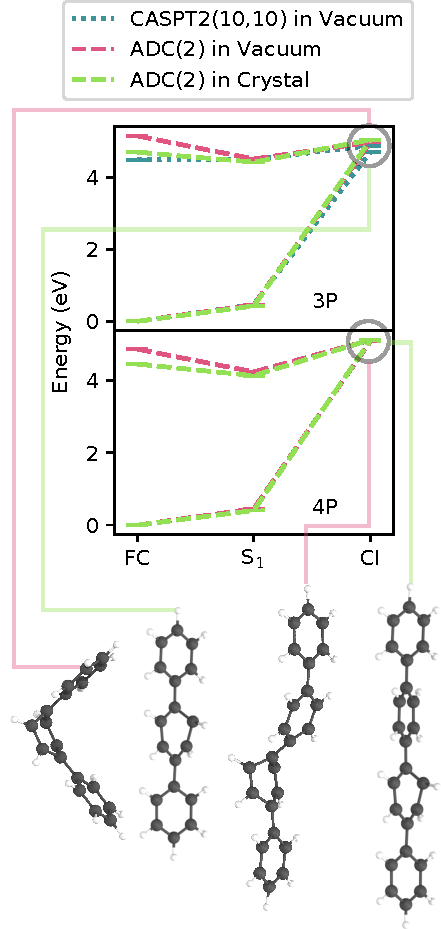
\includegraphics[width=6cm]{Chapters/7Applications/nP_conicals_master.pdf}
\caption{Energies of S$_0$ and S$_1$ states of 3P and 4P at the FC point, S$_1$ minima, and S$_1$\textendash{}S$_0$ MECI in vacuum (left) and crystal (right) computed at the RI-ADC(2)/def-SV(P) level. For the comparison, in the case of 3P, the corresponding CASPT2(10,10)/6-31G(d)//CASSCF(10,10)/6-31G(d) and CASPT2(8,8)/6-31G(d)//CASSCF(8,8)/6-31G(d) results are given}
\label{fig:nP_pathways}
\end{figure}

For both 3P and 4P, as shown in Figure \ref{fig:nP_pathways}, the optimised MECI geometries lie above the S$_1$ excitations at the FC point, both in vacuum and crystal, implying that this kind of internal conversion is inefficient for these systems. The energy of the 3P vacuum conical intersection, obtained with CASPT2(10,10)/6-31G(d)//CASSCF(10,10)/6-31G(d), lies 0.30 eV above the S$_1$ excitation at the FC point. ADC(2) successfully describes the region of the conical intersection of 3P and predicts the MECI energy close to the value obtained with CASPT2(10,10)/6-31G(d)//CASSCF(10,10)/6-31G(d), but it overestimates the vertical excitation at the FC region. In the case of 4P, the vacuum MECI optimised at the ADC(2)/def-SV(P) level is 0.24 eV above the S$_1$ state at the FC region.

For both systems, the optimised MECI structure in crystal is more energetic compared to the one in vacuum. The MECIs of 3P and 4P lie 0.34 eV and 0.67 eV above the excitation in the FC region, based on the ADC(2)/def-SV(P) optimisations.

The ADC(2)/def-SV(P) optimised MECI of 6P in vacuum corresponds to a puckering conical intersection with a prefulvene-like structure of the central ring. The rest of the chain is highly distorted due to rotation of terminal phenyl rings, as shown in Figure \ref{fig:6P_conical}.

\begin{figure}[h!]
\centering
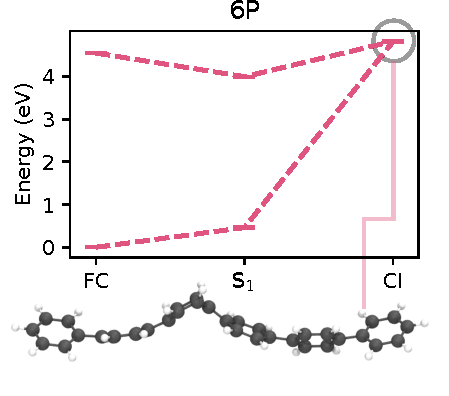
\includegraphics[width=5.8cm]{Chapters/7Applications/6P_conical.pdf}
\caption{Energies of S$_0$ and S$_1$ states of 6P at the FC point, S$_1$ minima, and S$_1$\textendash{}S$_0$ MECI in vacuum computed at the RI-ADC(2)/def-SV(P) level. The MECI structure is represented in the bottom.}
\label{fig:6P_conical}
\end{figure}

The S$_1$ state at the optimised vacuum S$_1$\textendash{}S$_0$ MECI is 0.18 eV above the vertical excitation at the FC point, implying that internal conversion is unfavourable for this molecule, as shown in Figure \ref{fig:6P_conical}. \miguel{The conical intersection optimisation in the crystal could only minimise the S$_1$\textendash{}$S_0$ gap to 0.3 eV, with an energy inversion between S$_1$ and S$_0$. This shows the inadequacy of single reference methods to characterise conical intersections in the case of 6P, which is also too large for computationally affordable and accurate multireference methods}. \mmiguel{However, multireference methods confirmed the accuracy of ADC(2) for 3P, so if we assume this to apply to 6P, then we observe a MECI energy several eV above the FC energy, making it inaccessible.}

Conical intersections are therefore rightly found to be at least partially inaccessible for 3P and 4P, bocking this nonradiative decay channel. However this barrier is even higher in 6P, which has lower QEF than 3P, indicating the importance of alternative nonradiative decay mechanisms for this crystal.

\miguel{Another explanation for the increased nonradiative decay rate of 6P due to internal conversion would be a vibrational nonradiative mechanism. This would be consistent with the lower S$_1$ energy of 6P, thus enabling large vibrational wavefunction overlap.} However, the low vibrational reorganisation energies of 3P and 6P are of the same order in solution and in crystal. The Supporting Information shows a reduction of these energies to 10\% upon crystallisation for both systems, which does not significantly impact the emissivity of 3P.


Stampfl \textit{et al.} proposed that the decrease of quantum efficiency upon aggregation in 6P is induced by intermolecular excitonic phenomena.\cite{6P_qy} This conclusion is based on a linearly decreasing luminescence efficiency with temperature, instead of an Arrhenius-type dependence. The former is explained by increased excitonic collision probabilities on higher temperatures, whereas the latter would be associated with intramolecular vibrational radiationless deactivation.

\mmiguel{Exciton hopping rates are quadratically dependent on the exciton coupling within a crystal, and inverse exponentially dependent on the reorganisation energy, as shown in Equation \ref{eq:marcus}. The exciton coupling in 6P crystals of 95 meV reported in Table \ref{tab:molecules} is of the same order as for 3P, with 98 meV. In contrast, the total reorganisation energy of 6P in crystal is 0.29 eV, compared to 3P's 0.35 eV, as can reported in Table \ref{tab:Rates}. This difference results in a hopping rate 1.95 greater in 6P than in 3P, a ratio approaching that of the different QEFs in crystal. We can postulate that an increased hopping rate leads to more nonradiative decay due to the mobile exciton more readily reaching surface, grain boundary, or bulk defects in the material}.

\mmiguel{In summary, vibrational and nonadiabatic nonradiative decay channels are mostly blocked in both vacuum and crystal for all members of this series.} The drop in QEF of 6P upon crystallisation is due to its particular property of displaying strong exciton couling, whilst having a low reorganisation energy compared to 3P. We can explain this property by the relative sparsity of 6P, with a steric volume index of 2.27 compared to 3P's 1.37, allowing for less strained reorganisation, but maintaining the high exciton coupling thanks to the length of the 3P backbone maximising $\pi$\textendash$\pi$ interactions.

\textbf{DCS Series}

Finally, we investigate the excited state decay channel of another aromatic molecule with a different structured backbone, based on the DSB molecule. $\alpha$-DCS is a DSB derivative displaying in impressive rise of QEF from 0.002 to 0.90 from solution to single crystal.\cite{Shi2017}

Its geometry was optimised in chloroform solvent using PCM to find its ground and excited state minima and conical intersection geometry. The results are shown on Figure \ref{fig:adcs}. The absorption energy was 3.84 eV, in close agreement with the experimental value of 3.80 eV. The FC minimum was characterised by a tilt of the inner ring with respect to the outer rings of 67.2\degree{}, whereas the S$_1$ optimisation led to a more planar geometry with an angle of 21.3\degree{}. This large reorganisation led to an emission energy of 2.84 eV, shifted 1.01 eV away from the absorption energy.

\begin{figure}
\centering
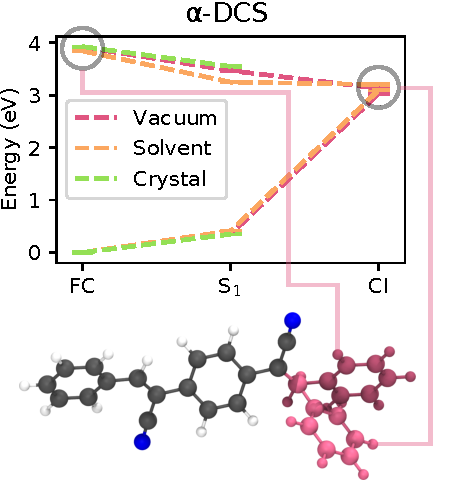
\includegraphics[width=5.8cm]{Chapters/7Applications/adcs.pdf}
\caption{$\alpha$-DCS energy at critical points of its excited state potential energy surface. The vacuum and solvent calculation used TD-$\omega$B97X-D/6-31G(d) and the crystal calculation TD-$\omega$B97X-D/6-31G(d):DFTB.}
\label{fig:adcs}
\end{figure}

The molecule was reoptimised in its crystal phase using OEEC. Here, the FC geometry had a tilt of 62.9\degree{} but the planarisation of S$_1$ was significantly hindered, only reaching 47.1\degree{}. We observe that the crystal packing reduces the flexibility of the molecule, which is calculated to absorb at 3.93 eV and emit at 3.20 eV, producing a Stokes shift of 0.73, a value smaller than in solution by 0.3 eV.

The increased rigidity also has implications for the geometry of the S$_1$\textendash{}S$_0$ MECI. The access to the conical intersection geometry in solvent for similar molecules has been characterised by a rotation about a double bond of the backbone, causing one ring to be on a perpendicular plane from the other two, and a pyramidalisation of the carbon connecting the rotated ring to the backbone.\cite{Izquierdo2019} We located a similar conical intersection for $\alpha$-DCS, where the rotation was of 88.8\degree{} about the same bond as reported in Reference \citenum{Izquierdo2019}, but involving no pyramidalisation. In either case, the rotation involved in the access to this S$_1$\textendash{}S$_0$ MECI supposes a large reorganisation which represent a quenched nonradiative decay channel in solution, and a blocked one in crystal. Indeed the crystal packing is too dense to allow for the backbone to draw an arc of nearly a right angle, instead the penalty function MECI optimisation algorithm pursues a double bond stretching CI too distorted to evaluate even with multireference methods.

Other emissive DSB-based molecules have similar molecular backbones and packing, as shown in Figure \ref{fig:angles}, pointing to a similar quenching of the internal conversion decay pathway. They have been investigated in a series of studies for their promising SSL properties.\cite{Shi2017,Shi2019,Izquierdo2019} They all have cyano-group (CN) substituents on the vinylene units which connect their phenylene rings. DBDCS and MODBDCS have additionally buthoxy-groups (OBu) on lateral phenylene rings at their para positions. Apart from CN- and OBu-substituents, the MODBDCS molecules are distinguished by methoxy-groups (OMe) on central phenylene rings in their meta positions. MODCS is characterised by OMe-substitutions on central phenylene rings. $\alpha$- and $\beta$-members of the series differ from each other by positions of CN- groups on vinylene units with respect to the phenylene rings; the former having CN- groups closer to the central ring, and the latter closer to lateral phenylene rings. 

\begin{table*}
\begin{tabular}{@{}lcccccccc@{}}
\toprule
\multirow{2}{*}{Molecule}   & \multirow{2}{*}{$k_r^{\text{sol}}$\cite{Shi2017}}  & \multirow{2}{*}{$k_{nr}^{\text{sol}}$\cite{Shi2017}} & \multirow{2}{*}{$\Phi_f^{\text{sol}}$\cite{Shi2017}} & \multirow{2}{*}{$\lambda^{\text{\text{vac}}}_{\text{low}}$} & \multirow{2}{*}{$k_r^{\text{cr}}$\cite{Shi2017}}   & \multirow{2}{*}{$k_{nr}^{\text{cr}}$\cite{Shi2017}} & \multirow{2}{*}{$\Phi_f^{\text{cr}}$\cite{Shi2017}} & \multirow{2}{*}{$\lambda^{\text{\text{cr}}}_{\text{low}}$}\\
\\
\midrule
$\alpha$-DCS     & 0.35 & 175  & 0.002 & 0.095 & 0.43 & 0.05 & 0.90 & 0.046 \\
$\alpha$-DBDCS   & 0.5  & 250  & 0.002 & 0.088 & 0.05 & 0.02 & 0.70 & 0.016 \\
$\beta$-DBDCS    & 0.45 & 0.39 & 0.54  & 0.090 & 0.14 & 0.03 & 0.84 & 0.035 \\
$\alpha$-MODCS   & 0.11 & 5.4  & 0.02  & 0.094 & 0.19 & 0.1  & 0.66 & 0.054 \\
$\beta$-MODCS    & 0.15 & 0.60 & 0.2   & 0.089 & 0.04 & 0.02 & 0.73 & 0.031 \\
$\alpha$-MODBDCS & 0.23 & 77   & 0.003 & 0.059 & 0.09 & 0.12 & 0.42 & 0.009  \\
$\beta$-MODBDCS  & 0.22 & 0.50 & 0.31  & 0.077 & 0.02 & 0.02 & 0.46 & 0.009  \\
\bottomrule
\end{tabular}
\caption{Experimental radiative rates in ns$^{-1}$ ($k_r$), nonradiative rates in ns$^{-1}$ ($k_{nr}$), luminescent efficiency ($\Phi_f$), and computed reorganisation energies for vibrational modes of less than 0.031 eV (250 cm$^{-1}$) in eV ($\lambda_{\text{low}}$) for the DCS series. The superscripts indicate the medium, where "sol" is chloroform solvent, "vac" is vacuum, and "cr" is single crystal}
%Experimental values of radiative rates (k$_r$ in $ns^{-1}$), nonradiative rates (k$_{nr}$ in $ns^{-1}$), fluorescence quantum yields ($\Phi_f$) in solution and aggregate phase.$^e$ Reference \citenum{Shi2017}}
\label{tab:Rates_DCS_series}
\end{table*}

All members of the series are emissive in the crystal form, with higher efficiency than in solution. In particular, the $\alpha$- systems are completely non-emissive in solution. As noted in the previous sections, changes in QEF are understood as a competing change in radiative and non-radiative rates, with the latter being contributed to by differing vibrational wavefunction overlap, intermolecular excitonic processes, and conical intersection accessibilities.

The nonradiative rates only increase upon aggregation for $\alpha$-DCS and $\alpha$-MODCS, as is reported in in Table \ref{tab:Rates_DCS_series}.\cite{Shi2017} Therefore, we can expect an important restriction of nonradiative decay mechanisms upon crystallisation for the series.

Regarding vibrational nonradiative decay, it has been proposed to contribute to SLE within the Restriction of Intramolecular Motions (RIM) model described in References \citenum{Shuai2014} and \citenum{Peng2007}. The crystallisation is said to quench low energy vibrational modes, thus impeding the overlap of vibrational wavefunctions between different excited states, and blocking Fermi-Golden-Rule-style nonradiative decay.

As is shown in Table \ref{tab:Rates_DCS_series} these modes are indeed reduced in the crystal phase for the DCS series, however less so than in 3P and 6P, whose nonradiatively decay is thought to principally be through conical intersections and excitonic dissipation. No clear trends emerge linking the quenching of vibrational modes upon crystallisation to the change in QEF of the systems, though they cannot be excluded as a contributing factor to the enhanced emission.

To probe for excitonic dissipation, we can focus on the case of the strongest coupled system, $\beta$-MODCS, as seen on Table \ref{tab:molecules}, with an exciton coupling of 140 meV. This does not impede a very efficient emission of 0.73, despite its low radiative rate reported in Table \ref{tab:Rates_DCS_series}. As shown in Figure \ref{fig:angles}, most crystals share the characteristic face-to-face dimer packing of sheet-like crystals, indicating that the character of their excitonic states should not be radically different. The principal exceptions are $\alpha$-DCS and $\alpha$-MODCS, where the former still displays the greatest crystal luminescent efficiency of the series, and the latter a mere 32 meV of exciton coupling. We can conclude that within this series, excitonic states are either present but not of a dissipative character, or absent.


% Both $\alpha$- and $\beta$-members of the series show SSLE. The $\alpha$-derivatives feature very low yields ($\Phi_f$) in solution, whereas fluorescence efficiencies of $\beta$-series are significant in solution, but are strongly dependent on a substituent type and position (they increase in order $\Phi$ ($\beta$-MODCS) = 0.20 < $\Phi$ ($\beta$-MODBDCS) = 0.31 < $\Phi$ ($\beta$-DBDCS) = 0.54.
% Even though the $\alpha$-derivatives of S$_1$ states have large oscillator strengths in solution, much faster internal conversion suppresses slower fluorescence.
% $\alpha$-derivatives have low emission in solution and significant emission in the solid state, whereas all $\beta$-derivatives are highly emissive in both phases. The increase on $\Phi_f$ due to both increase of $k_r$ and decrease of $k_{nr}$ happens only in $\alpha$-MODCS and in the rest of crystals $\Phi_f$ increases solely because of the decrease of $k_{nr}$ (Table \ref{tab:Rates_DCS_series}).[TEMPORARY PARAGRAPH]


As for the access to conical intersections, there is reported evidence for is importance in the series. Reference \citenum{Shi2019} observes a a rise in nonradiative decay rates with increasing FC energy in solution. This indicates the comparatively low importance of vibrational decay in the nonradiative rate of this family, due to a lesser overlap between ground and excited state vibrational wavefunctions in the low nonadiabatic coupling regime; leaving the RACI mechanism such as the one previously outlined for $\alpha$-DCS as the principal cause of SLE.\cite{Escudero2019}


The dominance of conical intersection decay in this series can also be linked to the low but present luminescence of the $\beta$- molecules in solution. The position of the CN- substituents upon the rotating section of the double bond which drives the access to the conical intersection, at least in $\alpha$-DCS, can constitute a hindrance to the the motion.

Moreover, the RACI model, depends on the rigidity of the molecules in the excited state, where a smaller conformational freedom of the molecule results in fewer pathways to the conical intersection to restrict. This is consistent with the overall greatest QEF, attributed to the smallest molecule\textemdash{}$\alpha$-DCS, with 0.90\textemdash{}and the lowest QEF to the ones with the most substituent\textemdash{}$\alpha$-MODBDCS and $\beta$-MODBDCS, with 0.42 and 0.46 respectively.



\section{Conclusions}

In this chapter, we have reviewed the crystalline excited state properties of thirteen organic molecular crystals with luminescent behaviour. We used a geometry analysis tool to characterise the different nearest neighbour dimers present in these crystals and associate them to particular crystal packing motifs. We observed that within one series of similar molecules\textendash{}DSB derivatives\textendash{}the packing motif determined the centroid-to-centroid distance of the resulting molecules.

This distance was shown to have direct implications as to the value of the exciton coupling between constituent fragments. Chemically different molecules were found to have similar exciton coupling values within a range of 50 meV. The weakness of this model was highlighted in the HBT crystal, where the centroid of the molecules is far away from the area with most electronic reorganisation upon excitation.

We also observed that the exciton coupling values accessible to dimers in their vibrational phase space are not particularly dependent on the intermolecular arrangement. Indeed the vibrations are mostly determined by the molecular structure, and dictate the broadness of values of the exciton coupling.

We then investigated the internal conversion decay channels for five of the crystals and how they were affected by their crystal environment. For these luminescent materials, the conical intersection energy was systematically found to be higher than the absorption energy, in crystal, pointing to a quenching due to steric hindrance. Molecules with rotation involved in their vacuum phase conical intersection were likelier to have a higher energy crystal conical intersection. In contrast, ones which had puckered geometries in vacuum found alternate puckering patterns in the crystal with close to equivalent energy profiles. \mmiguel{Clear links between the access to the conical intersection and the QEF were drawn for HBT and DCS systems. Vibrational decay was not directly shown to have a significant role in the darkness of any systems in the vacuum, and was further discouraged in the crystal by the quenching of low energy normal modes. Finally, excitonic dissipation was proposed as a determining mechanism explaining the different QEFs of the $n$P series.}

Overall, excited state decay mechanisms remain relatively system specific due to the formidable breadth of chemical space. \miguel{Fluorescence, internal conversion, and excitonic dissipation are competing mechanisms, interlinked by their relation to crystal structure. The complexity of this relationship is exemplified by the diverse luminescent behaviour in solution of the molecules in this study, despite their consistent efficient luminescence in as crystals.} \mmiguel{Programs like \texttt{fromage} prove themselves to be essential in disentangling the holistic mechanisms behind such phenomena.}


%%%%%%%%%%%%%%%%%%%%%%%%%%%%%%%%%%%

